\documentclass[sigconf,nonacm,screen]{acmart}
\usepackage{filecontents}
\usepackage{textcomp}
\usepackage{pgfplots}
\usetikzlibrary{patterns}
\usepackage{ifthen}
\usepgfplotslibrary{groupplots}
\RequirePackage{keyval}
\usepackage{multirow}
\usepackage{multicol}
\usepackage{csvsimple}
\usepackage[utf8]{inputenc}
\newcounter{row}
\newcounter{col}
\usepackage{wrapfig}
\usepackage{textgreek}
\usepackage[inline]{enumitem}
\usetikzlibrary{matrix, positioning}
\usetikzlibrary{patterns,tikzmark}
\usetikzlibrary{matrix,decorations.pathreplacing,calc}
\usepackage{hf-tikz}
\usepackage{pifont}
\usepackage{subfig}
\usetikzlibrary{chains,fit,shapes}
\usetikzlibrary{arrows.meta,
    chains,
    positioning,
    shapes.symbols}
\usetikzlibrary{decorations,calligraphy}
\usepackage{pgfplotstable}
\usepgfplotslibrary{statistics}
%\pgfplotsset{compat=newest}
\usetikzlibrary{matrix,calc}
\usetikzlibrary{fit}
\usepackage{xfp}
\usepackage{mathtools}

\usetikzlibrary{positioning}

\usepackage{makecell}
%\usepackage{tabu}
\usepackage{tikz}
\usetikzlibrary{trees}

%\pgfplotsset{compat=1.8}
\pgfplotsset{compat=1.12}


\usepgfplotslibrary{fillbetween}

\usepackage{filecontents}
% \usetikzlibrary{pgfplots.groupplots}
% \pgfplotsset{compat=1.9}

% \usepackage[utf8]{inputenc}
% \usepackage[ngerman]{babel}
% \usepackage{pgfplots}
% \pgfplotsset{compat=1.9}
% \usetikzlibrary{
%   pgfplots.groupplots,
%   matrix
% }
% \usepackage{siunitx}

\newtheorem{theorem}{Theorem}
\newtheorem{definition}{Definition}
\newcommand{\eat}[1]{}

\definecolor{bluegreen}{RGB}{3, 166, 155}
\definecolor{pitchblack}{RGB}{0, 0, 0}
\definecolor{lightbeige}{RGB}{255, 251, 241}
\definecolor{mediumgray}{RGB}{183, 183, 183}
\definecolor{mygreen}{rgb}{0,0.6,0}
\definecolor{mygray}{rgb}{0.5,0.5,0.5}
\definecolor{mymauve}{rgb}{0.58,0,0.82}
\definecolor{keywords}{RGB}{255,0,90}
\definecolor{comments}{RGB}{0,0,113}
\definecolor{red}{RGB}{255,0,0}
\definecolor{green}{RGB}{0,255,0}
\definecolor{navy}{RGB}{0,0,128}
\definecolor{DarkGrenen}{RGB}{0,100,0}
\definecolor{DarkOliveGreen}{RGB}{85,107,47}
\definecolor{saddlebrown}{RGB}{139,69,19}
\definecolor{gold}{RGB}{252,194,1}
\definecolor{tug}{RGB}{247,1,70}
\definecolor{tugb}{RGB}{120,137,251}


\definecolor{blue0}{RGB}{153,153,153}
\definecolor{blue1}{RGB}{77,77,77}%
\definecolor{blue2}{RGB}{165,71,209}
\definecolor{blue3}{RGB}{77,10,142}
\definecolor{blue4}{RGB}{74,139,203}
\definecolor{blue5}{RGB}{40,40,190}

\definecolor{color1}{RGB}{100,149,237} % corn flower blue
\definecolor{color2}{RGB}{153,153,153} % light gray
\definecolor{color3}{RGB}{0,0,0} % black
\definecolor{color4}{RGB}{255,165,0} % orange
\definecolor{color5}{RGB}{255,69,0} % orange red
\definecolor{color6}{RGB}{77,77,77} % dark gray
\definecolor{color7}{RGB}{31,119,180}
\definecolor{color8}{RGB}{7,77,125}
\definecolor{color9}{RGB}{153,216,201}


\definecolor{teal1}{RGB}{31, 111, 111}
\definecolor{teal2}{RGB}{84, 161, 161}
\definecolor{teal3}{RGB}{159, 200, 200}

\definecolor{dred1}{RGB}{160, 0, 0}
\definecolor{dred2}{RGB}{196, 102, 102}
\definecolor{dred3}{RGB}{216, 166, 166}


\definecolor{dblue1}{RGB}{32, 102, 168}
\definecolor{dblue2}{RGB}{53, 148, 204}
\definecolor{dblue3}{RGB}{140, 197, 227}

\definecolor{totalcolor}{RGB}{2, 152, 215}
\definecolor{mvcolor}{RGB}{248, 163, 47}
\definecolor{dvcolor}{RGB}{203, 70, 39}



% Enable this two commands when you want to extract diagrams in extra files, then run "make"
\usetikzlibrary{external}
\tikzexternalize[prefix=plots/] %  activate

\usetikzlibrary{positioning}

\sloppy
\clubpenalty = 10000
\widowpenalty = 10000
\brokenpenalty = 10000
\frenchspacing


\makeatletter
\def\pgfplots@drawaxis@lines@preparediscont@for#1{%
        \ifnum\csname pgfplots@#1axisdiscontnum\endcsname>0
                \begingroup
                % this group employs several temporary dimension registers
                % and is therefor scoped:
                \let\disstart=\pgf@ya
                \let\disend=\pgf@yb
                \disend=\csname pgfplots@#1max@reg\endcsname
                \advance\disend by -\csname pgfplots@#1min@reg\endcsname
                \disend=\csname pgfplots@#1@veclength\endcsname\disend
                \ifcase\csname pgfplots@#1axisdiscontnum\endcsname\relax
                        % has already been checked above.
                \or
                        \def\discontstyle{decoration={zigzag,segment length=5pt, amplitude=2pt}}%
                        \advance \disend by -8pt
                \or
                        \def\discontstyle{decoration={ticks,segment length=4pt, amplitude=8pt}}%
                        \advance \disend by -4pt
                \fi
                \pgfplotscoordmath{#1}{datascaletrafo get params}%
                % if #1max + shift < 0pt  (shift is 0 without the scaling trafo)
                \ifdim\csname pgfplots@#1max@reg\endcsname<-\pgfplotsretvalb pt
                        % swap start and end
                        \disstart=\disend
                        \disend=2pt
                \else
                        \disstart=2pt
                \fi
                % carry local computations outside of group:
                \xdef\pgfplots@glob@TMPa{%
                        \noexpand\def\expandafter\noexpand\csname #1disstart\endcsname{\the\disstart}%
                        \noexpand\def\expandafter\noexpand\csname #1disend\endcsname{\the\disend}%
                        \noexpand\pgfkeysdef{/tikz/#1discont}{\noexpand\pgfkeysalso{\discontstyle}}%
                }%
                \endgroup
                \pgfplots@glob@TMPa
        \else
                \expandafter\def\csname #1disstart\endcsname{0pt}%
                \expandafter\def\csname #1disend\endcsname{0pt}%
                \pgfkeyslet{/tikz/#1discont}=\pgfutil@empty
        \fi
}%
\makeatother



\begin{document}
\title[Query Processing by Data Catalog]{Query Processing by Data Catalog}

\author{Saeed Fathollahzadeh} 
\orcid{0000-0003-3723-6191}
\affiliation{
\institution{Concordia University}
\country{Canada}}

\renewcommand{\shortauthors}{Saeed Fathollahzadeh}

\maketitle

    % \tikzsetnextfilename{Experiment0-DataProfiling}
    % \begin{figure}[h]
    %     \centering
    %     \newcommand{\myaddplot}[1]{
  \addplot[fill=#1, draw=#1,line width=0.4pt] table[y=time, col sep=comma, x=dataset]{../archive/SIGMOD2025-Results/Experiment1-Profiling.dat};
  \label{total_time}    
};

\newcommand{\addplotreader}[1]{
\addplot[fill=#1, draw=#1,line width=0.4pt] table[y=time, col sep=comma, x=dataset]{../archive/SIGMOD2025-Results/Experiment1-DataReader.dat};
  \label{reader_time}    
};

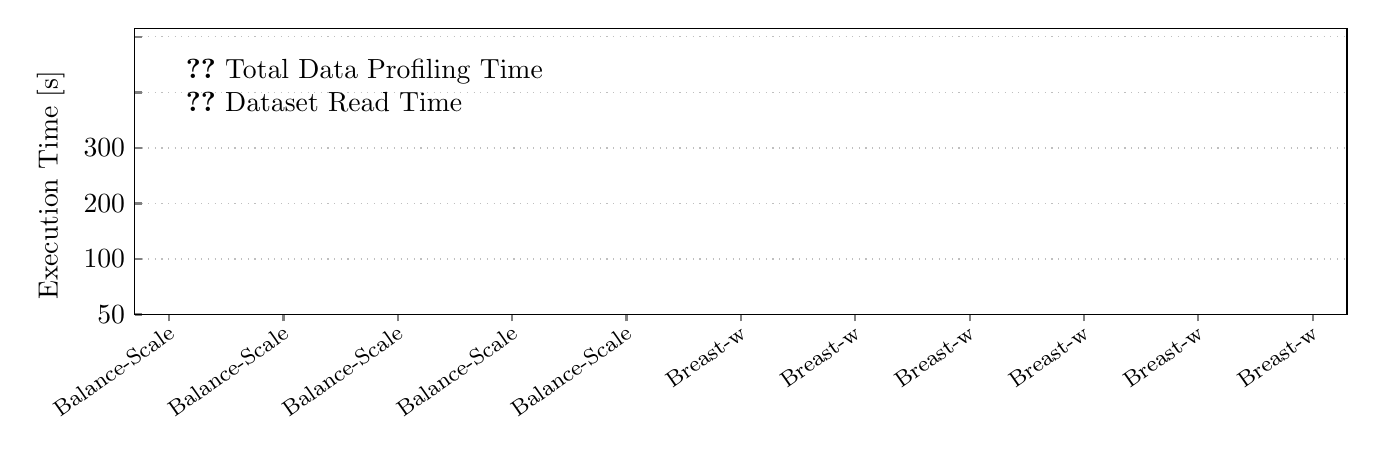
\begin{tikzpicture}[
  every axis/.style={
  height=0.43\columnwidth,
  width=1.4\columnwidth,  
  ymin=0,
  ymax=300000,
  }]
 \begin{axis}[   
  every major tick/.append style={ thick,major tick length=2.5pt, gray},
  axis line style={black},
  ybar,     
  log ticks with fixed point,
  y tick label style={/pgf/number format/1000 sep={}},
  x tick label style={/pgf/number format/1000 sep={}},
  scaled y ticks=false,
  enlarge y limits={0.03,upper},
  enlarge x limits=0.03,
  ylabel={Execution Time [s]},
  %xlabel={},
  ytick={0,50000,100000,200000,300000},
  yticklabels={0,50, 100, 200, 300},
  %xtick style={draw=none},
  xtick pos=left,
  ytick pos=left,
  yticklabel style = {font=\normalsize},
  ylabel style = {font=\normalsize, yshift=0pt, xshift=-5pt},
  xticklabel style = {font=\footnotesize, xshift=0pt, yshift=4pt, rotate=35, anchor=north east},
  ymajorgrids,
  grid style=dotted,
  minor grid style={gray!80, dotted},
  %nodes near coords,
  %every node near coord/.style={font=\fontsize{0.1pt}{0.1}, rotate=0},
  every axis plot/.append style={line width=0.8pt,mark options={scale=1.5,solid}},  
  legend image post style={line width=.5pt},  
  xtick = data,
  symbolic x coords={Balance-Scale,Breast-w,CMC,Credit-g,Diabetes,Tic-Tac-Toe,Eucalyptus,PC1,Jungle-Chess,Higgs,Skin,Traffic,Walking-Activity,Black-Friday,Bike-Sharing,House-Sales,NYC,Airlines-DepDelay},
  legend image code/.code={\draw [#1] (0cm,-0.1cm) rectangle (0.2cm,0.1cm); },  
%}
]  
  \myaddplot{tugb};

\end{axis}

\begin{axis}[
  axis y line*=right,
  axis x line=none,  
  ybar,        
  log ticks with fixed point,
  y tick label style={/pgf/number format/1000 sep={}},
  x tick label style={/pgf/number format/1000 sep={}},
  scaled y ticks=false,
  enlarge y limits={0.03,upper},
  enlarge x limits=0.03,
  ylabel={Execution Time [s]},
  ylabel={},
  xlabel={},
  ytick={},
  yticklabels={},
  ytick style={draw=none},
  yticklabel style = {font=\large},
  ylabel style = {font=\large, yshift=-3pt},
  xticklabel style = {font=\footnotesize, xshift=0pt, yshift=4pt, rotate=35, anchor=north east},
  %nodes near coords,
  %every node near coord/.style={font=\fontsize{0.1pt}{0.1}, rotate=0},
  every axis plot/.append style={line width=0.8pt,mark options={scale=1.5,solid}},  
  legend image post style={line width=.5pt},  
  xtick = data,
  symbolic x coords={Balance-Scale,Breast-w,CMC,Credit-g,Diabetes,Tic-Tac-Toe,Eucalyptus,PC1,Jungle-Chess,Higgs,Skin,Traffic,Walking-Activity,Black-Friday,Bike-Sharing,House-Sales,NYC,Airlines-DepDelay},
  legend image code/.code={\draw [#1] (0cm,-0.12cm) rectangle (0.25cm,0.12cm); }, 
  ]   
  \addplotreader{tug};
    
\end{axis}

\node [draw=none,inner sep=0, font=\normalsize, anchor=west] (leg1) at (rel axis cs: 0.07,0.80) {\shortstack[l]{
  \ref{total_time} Total Data Profiling Time \\
  \ref{reader_time} Dataset Read Time }};

\end{tikzpicture}
    %     \caption{DataProfiling}
    % \end{figure}  
    
    % \tikzsetnextfilename{Experiment0-Datasets-Overview}
    % \begin{figure}[h]
    %     \centering
    %     \newcommand{\addplotStatistics}[1]{
	   \addplot[xshift=0pt,draw=none,line width=0.15pt, fill=black]
	   table[ y=number_string, col sep=comma, x=dataset_name] {#1};
     \label{string}; 

     \addplot[xshift=0pt,draw=none,line width=0.15pt, fill=tug]
	   table[ y=number_int, col sep=comma, x=dataset_name] {#1};
     \label{int};  
     
     \addplot[xshift=0pt,draw=none,line width=0.15pt, fill=tugb]
	   table[ y=number_float, col sep=comma, x=dataset_name] {#1};
     \label{float};

     \addplot[xshift=0pt,draw=none,line width=0.15pt, fill=color4]
	   table[ y=number_bool, col sep=comma, x=dataset_name] {#1};
     \label{bool};
};

\begin{tikzpicture}[node distance=0mm]%
  \begin{groupplot}[
    group style={
        group name=my fancy plots,
        group size=2 by 1,
        %xticklabels at=edge bottom,
        horizontal sep=35pt,
        %height=.3\columnwidth,
    },
    every major tick/.append style={ thick,major tick length=2.5pt, gray},
    axis line style={black}, 
    enlarge y limits={0.03,upper},    
    ybar stacked,      
    log ticks with fixed point,
    %x tick label style={/pgf/number format/1000 sep={}},
    scaled y ticks=false,
    ylabel={Attribute's Count},
    xtick align=outside,
    xtick pos=left,
    ytick pos=left,
    yticklabel style = {font=\normalsize},
    ylabel style = {font=\normalsize, yshift=-3pt, xshift=-2pt},
    xticklabel style = {font=\footnotesize, xshift=0pt, yshift=4pt, rotate=35, anchor=north east},
    height=0.4\columnwidth,      
    ymajorgrids=true,
    grid style=dotted,   
    minor grid style={gray!50}, 
    xtick = data,
    %symbolic x coords={Nomao,Gas-Drift,Volkert,Black}, 
    legend image code/.code={\draw [#1] (0cm,-0.1cm) rectangle (0.2cm,0.1cm); }, 
]

\nextgroupplot[
  ymin=0,
  ymax=50,
  %xlabel style = {yshift=8pt, xshift=0pt},
  xlabel={},%{|Features| < 50},
  ytick={0,10,20,30,40,50},
  xtick = data,
  enlarge x limits=0.035,
  width=1\columnwidth,   
  symbolic x coords={Skin,Diabetes,Tic-Tac-Toe,Breast-w,Credit-g,Balance-Scale,Walking-Activity,Jungle-Chess,CMC,Higgs,Traffic,Black-Friday,Bike-Sharing,NYC,House-Sales}
]
\addplotStatistics{../archive/SIGMOD2025-Results/statistics/dataset_overview_small.dat}
%
\nextgroupplot[
  ymin=0,
  ymax=200,
  enlarge x limits=0.23,
  %xlabel style = {yshift=-6pt, xshift=0pt},
  xlabel={},%{|Features| > 100},  
  xtick = data,
  width=0.35\columnwidth,   
  symbolic x coords={Nomao,Gas-Drift,Volkert,Black}
]
\addplotStatistics{../archive/SIGMOD2025-Results/statistics/dataset_overview_large.dat}
\end{groupplot}
  \node [draw=none,inner sep=0, xshift=10pt, font=\normalsize, anchor=west] (leg1) at (rel axis cs: 1.1,1.07) {\shortstack[l]{
			\ref{string} String \ \ \ \  \ref{int} Int \ \ \ \  \ref{float} Float \ \ \ \  \ref{bool} Bool				 			
	}};

\end{tikzpicture}

    %     \caption{Datasets-Overview}
    % \end{figure} 
    
    %------------------------------    
  
    \tikzsetnextfilename{Statistics_Breast-w} 
        \begin{figure}[!ht]
            \centering
            \newcommand{\addplotStatistics}[1]{
	   \addplot+[draw=none,fill=dblue2 ]
	   table[ y=total_values_count, col sep=comma, x=col_index] {#1};
     \label{filled}; 

     \addplot+[draw=none, fill=mvcolor] 
	   table[ y=missing_values_count, col sep=comma, x=col_index] {#1};	   
	   \label{missed};       
};

\newcommand{\addplotDistinct}[1]{
	   \addplot[draw=none,fill=dred1 ]
	   table[ y=distinct_values_count, col sep=comma, x=col_index] {#1};
     \label{distinct};     
};

\begin{tikzpicture}[
  every axis/.style={
    %major x tick style = {draw=none},
    ybar stacked,    
    every major tick/.append style={ line width=0.5pt,major tick length=2pt, black},
    axis line style={draw=none},
    ymin=0,
    %xmin=1,
    xmax=10,
    ymax=699,
    tick label style={/pgf/number format/fixed},
    scaled y ticks=false,
    enlarge x limits=0.05,
    x tick label as interval=false,
    enlarge y limits=false,
    ylabel={},%{Samples},
    xlabel={\# Column},
    xtick={1,5,10},
    xticklabels={1,5,\hspace{-8pt}10},
    ytick={0,200,400,600,800,1000},
    yticklabels={0,200,400,600,800,1000},
    ytick align=outside,
    xtick align=outside,
    xtick pos=left,
    ytick pos=left,
    yticklabel style = {font=\normalsize},
    ylabel style = {yshift=-2pt},
    xticklabel style = {font=\normalsize, xshift=0pt},
    height=0.4\columnwidth,
    width=0.38\columnwidth,    
    bar width=4.8pt,	 
    %ymajorgrids=true,
    %grid style=dotted,   
    %minor grid style={gray!50}, 
    legend image code/.code={\draw [#1] (0cm,-0.1cm) rectangle (0.12cm,0.12cm); },
  }	 
]

\begin{axis}
  \addplotStatistics{../archive/VLDB2025/statistics/Breast-w_statistics.dat};	  	  
\end{axis}

\begin{axis} [hide axis]
  \addplotDistinct{../archive/VLDB2025/statistics/Breast-w_statistics.dat};	  	  
\end{axis}

% \node [draw=none,inner sep=0, font=\footnotesize, anchor=west] (leg1) at (rel axis cs: -0.65,1.16) {\shortstack[l]{
%   \ref{filled} Value 
%   \ref{missed} Missed 
%   \ref{distinct} Distinct		 			
% }};

\end{tikzpicture}

            \caption{Breast-w}
        \end{figure}  
    
  
    \tikzsetnextfilename{Statistics_CMC} 
        \begin{figure}[!ht]
            \centering
            \newcommand{\addplotStatistics}[1]{
	   \addplot+[draw=color7,line width=0.15pt, fill=color7 ]
	   table[ y=total_values_count, col sep=comma, x=col_index] {#1};
     \label{filled}; 

     \addplot+[draw=color4,line width=0.15pt, fill=color4] 
	   table[ y=missing_values_count, col sep=comma, x=col_index] {#1};	   
	   \label{missed};       
};

\newcommand{\addplotDistinct}[1]{
	   \addplot[draw=black,line width=0.15pt, fill=black ]
	   table[ y=distinct_values_count, col sep=comma, x=col_index] {#1};
     \label{distinct};     
};

\begin{tikzpicture}[
  every axis/.style={
    %major x tick style = {draw=none},
    ybar stacked,    
    every major tick/.append style={ thick,major tick length=2.5pt, gray},
    axis line style={gray},
    ymin=0,
    %xmin=1,
    xmax=10,
    ymax=1473,
    tick label style={/pgf/number format/fixed},
    %y tick label style={/pgf/number format/1000 sep={}},
    %x tick label style={/pgf/number format/1000 sep={}},
    scaled y ticks=false,
    %enlarge y limits={0.013,upper},
    enlarge x limits=0.02,
    x tick label as interval=false,
    enlarge y limits=false,
    ylabel={Samples},
    xlabel={\# Column},
    xtick={2,4,6,8,10},
    ytick={0,300,600,900,1200,1500},
    yticklabels={0,300,600,900,1200,1500},
    ytick align=outside,
    xtick align=outside,
    xtick pos=left,
    ytick pos=left,
    yticklabel style = {font=\normalsize},
    ylabel style = {yshift=-2pt},
    xticklabel style = {font=\normalsize, xshift=0pt},
    height=0.4\columnwidth,
    width=0.38\columnwidth,    
    bar width=0.03333333333333333\columnwidth,	 
    %ymajorgrids=true,
    %grid style=dotted,   
    %minor grid style={gray!50}, 
    legend image code/.code={\draw [#1] (0cm,-0.1cm) rectangle (0.12cm,0.12cm); },
  }	 
]

\begin{axis}
  \addplotStatistics{../archive/SIGMOD2025-Results/statistics/CMC_statistics.dat};	  	  
\end{axis}

\begin{axis} [hide axis]
  \addplotDistinct{../archive/SIGMOD2025-Results/statistics/CMC_statistics.dat};	  	  
\end{axis}

\node [draw=none,inner sep=0, font=\footnotesize, anchor=west] (leg1) at (rel axis cs: -0.65,1.16) {\shortstack[l]{
  \ref{filled} Value 
  \ref{missed} Missed 
  \ref{distinct} Distinct		 			
}};

\end{tikzpicture}

            \caption{CMC}
        \end{figure}  
    
  
    \tikzsetnextfilename{Statistics_Credit-g} 
        \begin{figure}[!ht]
            \centering
            \newcommand{\addplotStatistics}[1]{
	   \addplot+[draw=none,fill=dblue2 ]
	   table[ y=total_values_count, col sep=comma, x=col_index] {#1};
     \label{filled}; 

     \addplot+[draw=none, fill=mvcolor] 
	   table[ y=missing_values_count, col sep=comma, x=col_index] {#1};	   
	   \label{missed};       
};

\newcommand{\addplotDistinct}[1]{
	   \addplot[draw=none,fill=dred1 ]
	   table[ y=distinct_values_count, col sep=comma, x=col_index] {#1};
     \label{distinct};     
};

\begin{tikzpicture}[
  every axis/.style={
    %major x tick style = {draw=none},
    ybar stacked,    
    every major tick/.append style={ line width=0.5pt,major tick length=2pt, black},
    axis line style={draw=none},
    ymin=0,
    %xmin=1,
    xmax=21,
    ymax=1000,
    tick label style={/pgf/number format/fixed},
    scaled y ticks=false,
    enlarge x limits=0.02,
    x tick label as interval=false,
    enlarge y limits=false,
    ylabel={},%{Samples},
    xlabel={\# Column},
    xtick={1,10,20},
    xticklabels={1,10,\hspace{-5pt}20},
    ytick={0,300,600,900},
    yticklabels={0,300,600,900},
    ytick align=outside,
    xtick align=outside,
    xtick pos=left,
    ytick pos=left,
    yticklabel style = {font=\normalsize},
    ylabel style = {yshift=-2pt},
    xticklabel style = {font=\normalsize, xshift=0pt},
    height=0.4\columnwidth,
    width=0.38\columnwidth,    
    bar width=2.3pt,	 
    %ymajorgrids=true,
    %grid style=dotted,   
    %minor grid style={gray!50}, 
    legend image code/.code={\draw [#1] (0cm,-0.1cm) rectangle (0.12cm,0.12cm); },
  }	 
]

\begin{axis}
  \addplotStatistics{../archive/VLDB2025/statistics/Credit-g_statistics.dat};	  	  
\end{axis}

\begin{axis} [hide axis]
  \addplotDistinct{../archive/VLDB2025/statistics/Credit-g_statistics.dat};	  	  
\end{axis}

% \node [draw=none,inner sep=0, font=\footnotesize, anchor=west] (leg1) at (rel axis cs: -0.65,1.16) {\shortstack[l]{
%   \ref{filled} Value 
%   \ref{missed} Missed 
%   \ref{distinct} Distinct		 			
% }};

\end{tikzpicture}

            \caption{Credit-g}
        \end{figure}  
    
  
    \tikzsetnextfilename{Statistics_Diabetes} 
        \begin{figure}[!ht]
            \centering
            \newcommand{\addplotStatistics}[1]{
	   \addplot+[draw=color7,line width=0.15pt, fill=color7 ]
	   table[ y=total_values_count, col sep=comma, x=col_index] {#1};
     \label{filled}; 

     \addplot+[draw=color4,line width=0.15pt, fill=color4] 
	   table[ y=missing_values_count, col sep=comma, x=col_index] {#1};	   
	   \label{missed};       
};

\newcommand{\addplotDistinct}[1]{
	   \addplot[draw=black,line width=0.15pt, fill=black ]
	   table[ y=distinct_values_count, col sep=comma, x=col_index] {#1};
     \label{distinct};     
};

\begin{tikzpicture}[
  every axis/.style={
    %major x tick style = {draw=none},
    ybar stacked,    
    every major tick/.append style={ thick,major tick length=2.5pt, gray},
    axis line style={gray},
    ymin=0,
    %xmin=1,
    xmax=9,
    ymax=768,
    tick label style={/pgf/number format/fixed},
    %y tick label style={/pgf/number format/1000 sep={}},
    %x tick label style={/pgf/number format/1000 sep={}},
    scaled y ticks=false,
    %enlarge y limits={0.013,upper},
    enlarge x limits=0.02,
    x tick label as interval=false,
    enlarge y limits=false,
    ylabel={Samples},
    xlabel={\# Column},
    xtick={1,2,3,4,5,6,7,8,9},
    ytick={0,200,400,600,800,1000},
    yticklabels={0,200,400,600,800,1000},
    ytick align=outside,
    xtick align=outside,
    xtick pos=left,
    ytick pos=left,
    yticklabel style = {font=\normalsize},
    ylabel style = {yshift=-2pt},
    xticklabel style = {font=\normalsize, xshift=0pt},
    height=0.4\columnwidth,
    width=0.38\columnwidth,    
    bar width=0.037037037037037035\columnwidth,	 
    %ymajorgrids=true,
    %grid style=dotted,   
    %minor grid style={gray!50}, 
    legend image code/.code={\draw [#1] (0cm,-0.1cm) rectangle (0.12cm,0.12cm); },
  }	 
]

\begin{axis}
  \addplotStatistics{../archive/SIGMOD2025-Results/statistics/Diabetes_statistics.dat};	  	  
\end{axis}

\begin{axis} [hide axis]
  \addplotDistinct{../archive/SIGMOD2025-Results/statistics/Diabetes_statistics.dat};	  	  
\end{axis}

\node [draw=none,inner sep=0, font=\footnotesize, anchor=west] (leg1) at (rel axis cs: -0.65,1.16) {\shortstack[l]{
  \ref{filled} Value 
  \ref{missed} Missed 
  \ref{distinct} Distinct		 			
}};

\end{tikzpicture}

            \caption{Diabetes}
        \end{figure}  
    
  
    \tikzsetnextfilename{Statistics_Tic-Tac-Toe} 
        \begin{figure}[!ht]
            \centering
            \newcommand{\addplotStatistics}[1]{
	   \addplot+[draw=color7,line width=0.15pt, fill=color7 ]
	   table[ y=total_values_count, col sep=comma, x=col_index] {#1};
     \label{filled}; 

     \addplot+[draw=color4,line width=0.15pt, fill=color4] 
	   table[ y=missing_values_count, col sep=comma, x=col_index] {#1};	   
	   \label{missed};       
};

\newcommand{\addplotDistinct}[1]{
	   \addplot[draw=black,line width=0.15pt, fill=black ]
	   table[ y=distinct_values_count, col sep=comma, x=col_index] {#1};
     \label{distinct};     
};

\begin{tikzpicture}[
  every axis/.style={
    %major x tick style = {draw=none},
    ybar stacked,    
    every major tick/.append style={ thick,major tick length=2.5pt, gray},
    axis line style={gray},
    ymin=0,
    %xmin=1,
    xmax=10,
    ymax=958,
    tick label style={/pgf/number format/fixed},
    %y tick label style={/pgf/number format/1000 sep={}},
    %x tick label style={/pgf/number format/1000 sep={}},
    scaled y ticks=false,
    %enlarge y limits={0.013,upper},
    enlarge x limits=0.02,
    x tick label as interval=false,
    enlarge y limits=false,
    ylabel={Samples},
    xlabel={\# Column},
    xtick={2,4,6,8,10},
    ytick={0,200,400,600,800,1000},
    yticklabels={0,200,400,600,800,1000},
    ytick align=outside,
    xtick align=outside,
    xtick pos=left,
    ytick pos=left,
    yticklabel style = {font=\normalsize},
    ylabel style = {yshift=-2pt},
    xticklabel style = {font=\normalsize, xshift=0pt},
    height=0.4\columnwidth,
    width=0.38\columnwidth,    
    bar width=0.03333333333333333\columnwidth,	 
    %ymajorgrids=true,
    %grid style=dotted,   
    %minor grid style={gray!50}, 
    legend image code/.code={\draw [#1] (0cm,-0.1cm) rectangle (0.12cm,0.12cm); },
  }	 
]

\begin{axis}
  \addplotStatistics{../archive/SIGMOD2025-Results/statistics/Tic-Tac-Toe_statistics.dat};	  	  
\end{axis}

\begin{axis} [hide axis]
  \addplotDistinct{../archive/SIGMOD2025-Results/statistics/Tic-Tac-Toe_statistics.dat};	  	  
\end{axis}

\node [draw=none,inner sep=0, font=\footnotesize, anchor=west] (leg1) at (rel axis cs: -0.65,1.16) {\shortstack[l]{
  \ref{filled} Value 
  \ref{missed} Missed 
  \ref{distinct} Distinct		 			
}};

\end{tikzpicture}

            \caption{Tic-Tac-Toe}
        \end{figure}  
    
    \tikzsetnextfilename{Statistics_Nomao} 
    \begin{figure}[!ht]
        \centering
        \newcommand{\addplotStatistics}[1]{
	   \addplot+[draw=none,fill=dblue2 ]
	   table[ y=total_values_count, col sep=comma, x=col_index] {#1};
     \label{filled}; 

     \addplot+[draw=none, fill=mvcolor] 
	   table[ y=missing_values_count, col sep=comma, x=col_index] {#1};	   
	   \label{missed};       
};

\newcommand{\addplotDistinct}[1]{
	   \addplot[draw=none,fill=dred1 ]
	   table[ y=distinct_values_count, col sep=comma, x=col_index] {#1};
     \label{distinct};     
};

\begin{tikzpicture}[
  every axis/.style={
    %major x tick style = {draw=none},
    ybar stacked,    
    every major tick/.append style={ line width=0.5pt,major tick length=2pt, black},
    axis line style={draw=none},
    ymin=0,
    %xmin=1,
    xmax=119,
    ymax=34465,
    tick label style={/pgf/number format/fixed},
    scaled y ticks=false,
    enlarge x limits=0.01,
    x tick label as interval=false,
    enlarge y limits=false,
    ylabel={},%{Samples},
    xlabel={\# Column},
    xtick={1,50,100},
    ytick={0,10000,20000,30000,40000,50000},
    yticklabels={0,1e4,2e4,3e4,4e4,5e4},
    ytick align=outside,
    xtick align=outside,
    xtick pos=left,
    ytick pos=left,
    yticklabel style = {font=\normalsize},
    ylabel style = {yshift=-2pt},
    xticklabel style = {font=\normalsize, xshift=0pt},
    height=0.4\columnwidth,
    width=0.38\columnwidth,    
    bar width=0.5pt,	 
    %ymajorgrids=true,
    %grid style=dotted,   
    %minor grid style={gray!50}, 
    legend image code/.code={\draw [#1] (0cm,-0.1cm) rectangle (0.12cm,0.12cm); },
  }	 
]

\begin{axis}
  \addplotStatistics{../archive/VLDB2025/statistics/Nomao_statistics.dat};	  	  
\end{axis}

\begin{axis} [hide axis]
  \addplotDistinct{../archive/VLDB2025/statistics/Nomao_statistics.dat};	  	  
\end{axis}

% \node [draw=none,inner sep=0, font=\footnotesize, anchor=west] (leg1) at (rel axis cs: -0.65,1.16) {\shortstack[l]{
%   \ref{filled} Value 
%   \ref{missed} Missed 
%   \ref{distinct} Distinct		 			
% }};

\end{tikzpicture}

        \caption{Nomao}
    \end{figure}  


\tikzsetnextfilename{Statistics_Volkert} 
    \begin{figure}[!ht]
        \centering
        \newcommand{\addplotStatistics}[1]{
	   \addplot+[draw=color7,line width=0.15pt, fill=color7 ]
	   table[ y=total_values_count, col sep=comma, x=col_index] {#1};
     \label{filled}; 

     \addplot+[draw=color4,line width=0.15pt, fill=color4] 
	   table[ y=missing_values_count, col sep=comma, x=col_index] {#1};	   
	   \label{missed};       
};

\newcommand{\addplotDistinct}[1]{
	   \addplot[draw=black,line width=0.15pt, fill=black ]
	   table[ y=distinct_values_count, col sep=comma, x=col_index] {#1};
     \label{distinct};     
};

\begin{tikzpicture}[
  every axis/.style={
    %major x tick style = {draw=none},
    ybar stacked,    
    every major tick/.append style={ thick,major tick length=2.5pt, gray},
    axis line style={gray},
    ymin=0,
    %xmin=1,
    xmax=181,
    ymax=58310,
    tick label style={/pgf/number format/fixed},
    %y tick label style={/pgf/number format/1000 sep={}},
    %x tick label style={/pgf/number format/1000 sep={}},
    scaled y ticks=false,
    %enlarge y limits={0.013,upper},
    enlarge x limits=0.02,
    x tick label as interval=false,
    enlarge y limits=false,
    ylabel={Samples},
    xlabel={\# Column},
    xtick={1,50,100,150,200},
    ytick={0,10000,20000,30000,40000,50000,60000},
    yticklabels={0,1e4,2e4,3e4,4e4,5e4,6e4},
    ytick align=outside,
    xtick align=outside,
    xtick pos=left,
    ytick pos=left,
    yticklabel style = {font=\normalsize},
    ylabel style = {yshift=-2pt},
    xticklabel style = {font=\normalsize, xshift=0pt},
    height=0.4\columnwidth,
    width=0.38\columnwidth,    
    bar width=0.0018416206261510127\columnwidth,	 
    %ymajorgrids=true,
    %grid style=dotted,   
    %minor grid style={gray!50}, 
    legend image code/.code={\draw [#1] (0cm,-0.1cm) rectangle (0.12cm,0.12cm); },
  }	 
]

\begin{axis}
  \addplotStatistics{../archive/SIGMOD2025-Results/statistics/Volkert_statistics.dat};	  	  
\end{axis}

\begin{axis} [hide axis]
  \addplotDistinct{../archive/SIGMOD2025-Results/statistics/Volkert_statistics.dat};	  	  
\end{axis}

\node [draw=none,inner sep=0, font=\footnotesize, anchor=west] (leg1) at (rel axis cs: -0.65,1.16) {\shortstack[l]{
  \ref{filled} Value 
  \ref{missed} Missed 
  \ref{distinct} Distinct		 			
}};

\end{tikzpicture}

        \caption{Volkert}
    \end{figure}  


\tikzsetnextfilename{Statistics_Gas-Drift} 
    \begin{figure}[!ht]
        \centering
        \newcommand{\addplotStatistics}[1]{
	   \addplot+[draw=none,fill=dblue2 ]
	   table[ y=total_values_count, col sep=comma, x=col_index] {#1};
     \label{filled}; 

     \addplot+[draw=none, fill=mvcolor] 
	   table[ y=missing_values_count, col sep=comma, x=col_index] {#1};	   
	   \label{missed};       
};

\newcommand{\addplotDistinct}[1]{
	   \addplot[draw=none,fill=dred1 ]
	   table[ y=distinct_values_count, col sep=comma, x=col_index] {#1};
     \label{distinct};     
};

\begin{tikzpicture}[
  every axis/.style={
    %major x tick style = {draw=none},
    ybar stacked,    
    every major tick/.append style={ line width=0.5pt,major tick length=2pt, black},
    axis line style={draw=none},
    ymin=0,
    %xmin=1,
    xmax=129,
    ymax=13910,
    tick label style={/pgf/number format/fixed},
    scaled y ticks=false,
    enlarge x limits=0.005,
    x tick label as interval=false,
    enlarge y limits=false,
    ylabel={},%{Samples},
    xlabel={\# Column},
    xtick={1,50,100},
    ytick={0,4000,8000,12000},
    yticklabels={0,4e3,8e3,12e3},
    ytick align=outside,
    xtick align=outside,
    xtick pos=left,
    ytick pos=left,
    yticklabel style = {font=\normalsize},
    ylabel style = {yshift=-2pt},
    xticklabel style = {font=\normalsize, xshift=0pt},
    height=0.4\columnwidth,
    width=0.38\columnwidth,    
    bar width=0.3pt,	 
    %ymajorgrids=true,
    %grid style=dotted,   
    %minor grid style={gray!50}, 
    legend image code/.code={\draw [#1] (0cm,-0.1cm) rectangle (0.12cm,0.12cm); },
  }	 
]

\begin{axis}
  \addplotStatistics{../archive/VLDB2025/statistics/Gas-Drift_statistics.dat};	  	  
\end{axis}

\begin{axis} [hide axis]
  \addplotDistinct{../archive/VLDB2025/statistics/Gas-Drift_statistics.dat};	  	  
\end{axis}

% \node [draw=none,inner sep=0, font=\footnotesize, anchor=west] (leg1) at (rel axis cs: -0.65,1.16) {\shortstack[l]{
%   \ref{filled} Value 
%   \ref{missed} Missed 
%   \ref{distinct} Distinct		 			
% }};

\end{tikzpicture}

        \caption{Gas-Drift}
    \end{figure}  
    
  
    \tikzsetnextfilename{Statistics_Jungle-Chess} 
        \begin{figure}[!ht]
            \centering
            \newcommand{\addplotStatistics}[1]{
	   \addplot+[draw=color7,line width=0.15pt, fill=color7 ]
	   table[ y=total_values_count, col sep=comma, x=col_index] {#1};
     \label{filled}; 

     \addplot+[draw=color4,line width=0.15pt, fill=color4] 
	   table[ y=missing_values_count, col sep=comma, x=col_index] {#1};	   
	   \label{missed};       
};

\newcommand{\addplotDistinct}[1]{
	   \addplot[draw=black,line width=0.15pt, fill=black ]
	   table[ y=distinct_values_count, col sep=comma, x=col_index] {#1};
     \label{distinct};     
};

\begin{tikzpicture}[
  every axis/.style={
    %major x tick style = {draw=none},
    ybar stacked,    
    every major tick/.append style={ thick,major tick length=2.5pt, gray},
    axis line style={gray},
    ymin=0,
    %xmin=1,
    xmax=7,
    ymax=44819,
    tick label style={/pgf/number format/fixed},
    %y tick label style={/pgf/number format/1000 sep={}},
    %x tick label style={/pgf/number format/1000 sep={}},
    scaled y ticks=false,
    %enlarge y limits={0.013,upper},
    enlarge x limits=0.02,
    x tick label as interval=false,
    enlarge y limits=false,
    ylabel={Samples},
    xlabel={\# Column},
    xtick={1,2,3,4,5,6,7,8,9},
    ytick={0,10000,20000,30000,40000,50000},
    yticklabels={0,1e4,2e4,3e4,4e4,5e4},
    ytick align=outside,
    xtick align=outside,
    xtick pos=left,
    ytick pos=left,
    yticklabel style = {font=\normalsize},
    ylabel style = {yshift=-2pt},
    xticklabel style = {font=\normalsize, xshift=0pt},
    height=0.4\columnwidth,
    width=0.38\columnwidth,    
    bar width=0.047619047619047616\columnwidth,	 
    %ymajorgrids=true,
    %grid style=dotted,   
    %minor grid style={gray!50}, 
    legend image code/.code={\draw [#1] (0cm,-0.1cm) rectangle (0.12cm,0.12cm); },
  }	 
]

\begin{axis}
  \addplotStatistics{../archive/SIGMOD2025-Results/statistics/Jungle-Chess_statistics.dat};	  	  
\end{axis}

\begin{axis} [hide axis]
  \addplotDistinct{../archive/SIGMOD2025-Results/statistics/Jungle-Chess_statistics.dat};	  	  
\end{axis}

\node [draw=none,inner sep=0, font=\footnotesize, anchor=west] (leg1) at (rel axis cs: -0.65,1.16) {\shortstack[l]{
  \ref{filled} Value 
  \ref{missed} Missed 
  \ref{distinct} Distinct		 			
}};

\end{tikzpicture}

            \caption{Jungle-Chess}
        \end{figure}  
    
  
    \tikzsetnextfilename{Statistics_Higgs} 
        \begin{figure}[!ht]
            \centering
            \newcommand{\addplotStatistics}[1]{
	   \addplot+[draw=color7,line width=0.15pt, fill=color7 ]
	   table[ y=total_values_count, col sep=comma, x=col_index] {#1};
     \label{filled}; 

     \addplot+[draw=color4,line width=0.15pt, fill=color4] 
	   table[ y=missing_values_count, col sep=comma, x=col_index] {#1};	   
	   \label{missed};       
};

\newcommand{\addplotDistinct}[1]{
	   \addplot[draw=black,line width=0.15pt, fill=black ]
	   table[ y=distinct_values_count, col sep=comma, x=col_index] {#1};
     \label{distinct};     
};

\begin{tikzpicture}[
  every axis/.style={
    %major x tick style = {draw=none},
    ybar stacked,    
    every major tick/.append style={ thick,major tick length=2.5pt, gray},
    axis line style={gray},
    ymin=0,
    %xmin=1,
    xmax=29,
    ymax=11000000,
    tick label style={/pgf/number format/fixed},
    %y tick label style={/pgf/number format/1000 sep={}},
    %x tick label style={/pgf/number format/1000 sep={}},
    scaled y ticks=false,
    %enlarge y limits={0.013,upper},
    enlarge x limits=0.02,
    x tick label as interval=false,
    enlarge y limits=false,
    ylabel={Samples},
    xlabel={\# Column},
    xtick={1,6,12,18,24,30},
    ytick={0,2000000,4000000, 6000000, 8000000, 10000000},
    yticklabels={0,2e6,4e6,6e6,8e6, 10e6},
    ytick align=outside,
    xtick align=outside,
    xtick pos=left,
    ytick pos=left,
    yticklabel style = {font=\normalsize},
    ylabel style = {yshift=-2pt},
    xticklabel style = {font=\normalsize, xshift=0pt},
    height=0.4\columnwidth,
    width=0.38\columnwidth,    
    bar width=0.011494252873563218\columnwidth,	 
    %ymajorgrids=true,
    %grid style=dotted,   
    %minor grid style={gray!50}, 
    legend image code/.code={\draw [#1] (0cm,-0.1cm) rectangle (0.12cm,0.12cm); },
  }	 
]

\begin{axis}
  \addplotStatistics{../archive/SIGMOD2025-Results/statistics/Higgs_statistics.dat};	  	  
\end{axis}

\begin{axis} [hide axis]
  \addplotDistinct{../archive/SIGMOD2025-Results/statistics/Higgs_statistics.dat};	  	  
\end{axis}

\node [draw=none,inner sep=0, font=\footnotesize, anchor=west] (leg1) at (rel axis cs: -0.65,1.16) {\shortstack[l]{
  \ref{filled} Value 
  \ref{missed} Missed 
  \ref{distinct} Distinct		 			
}};

\end{tikzpicture}

            \caption{Higgs}
        \end{figure}  
    
  
    \tikzsetnextfilename{Statistics_Skin} 
        \begin{figure}[!ht]
            \centering
            \newcommand{\addplotStatistics}[1]{
	   \addplot+[draw=none,fill=dblue2 ]
	   table[ y=total_values_count, col sep=comma, x=col_index] {#1};
     \label{filled}; 

     \addplot+[draw=none, fill=mvcolor] 
	   table[ y=missing_values_count, col sep=comma, x=col_index] {#1};	   
	   \label{missed};       
};

\newcommand{\addplotDistinct}[1]{
	   \addplot[draw=none,fill=dred1 ]
	   table[ y=distinct_values_count, col sep=comma, x=col_index] {#1};
     \label{distinct};     
};

\begin{tikzpicture}[
  every axis/.style={
    %major x tick style = {draw=none},
    ybar stacked,    
    every major tick/.append style={ line width=0.5pt,major tick length=2pt, black},
    axis line style={draw=none},
    ymin=0,
    %xmin=1,
    xmax=4,
    ymax=245057,
    tick label style={/pgf/number format/fixed},
    scaled y ticks=false,
    enlarge x limits=0.15,
    x tick label as interval=false,
    enlarge y limits=false,
    ylabel={},%{Samples},
    xlabel={\# Column},
    xtick={1,2,3,4},
    ytick={0,50000,100000,150000,200000},
    yticklabels={0,5e5,10e5,15e5,20e5},
    ytick align=outside,
    xtick align=outside,
    xtick pos=left,
    ytick pos=left,
    yticklabel style = {font=\normalsize},
    ylabel style = {yshift=-2pt},
    xticklabel style = {font=\normalsize, xshift=0pt},
    height=0.4\columnwidth,
    width=0.38\columnwidth,    
    bar width=12pt,	 
    %ymajorgrids=true,
    %grid style=dotted,   
    %minor grid style={gray!50}, 
    legend image code/.code={\draw [#1] (0cm,-0.1cm) rectangle (0.12cm,0.12cm); },
  }	 
]

\begin{axis}
  \addplotStatistics{../archive/VLDB2025/statistics/Skin_statistics.dat};	  	  
\end{axis}

\begin{axis} [hide axis]
  \addplotDistinct{../archive/VLDB2025/statistics/Skin_statistics.dat};	  	  
\end{axis}

% \node [draw=none,inner sep=0, font=\footnotesize, anchor=west] (leg1) at (rel axis cs: -0.65,1.16) {\shortstack[l]{
%   \ref{filled} Value 
%   \ref{missed} Missed 
%   \ref{distinct} Distinct		 			
% }};

\end{tikzpicture}

            \caption{Skin}
        \end{figure}  
    
  
    \tikzsetnextfilename{Statistics_Traffic} 
        \begin{figure}[!ht]
            \centering
            \newcommand{\addplotStatistics}[1]{
	   \addplot+[draw=color7,line width=0.15pt, fill=color7 ]
	   table[ y=total_values_count, col sep=comma, x=col_index] {#1};
     \label{filled}; 

     \addplot+[draw=color4,line width=0.15pt, fill=color4] 
	   table[ y=missing_values_count, col sep=comma, x=col_index] {#1};	   
	   \label{missed};       
};

\newcommand{\addplotDistinct}[1]{
	   \addplot[draw=black,line width=0.15pt, fill=black ]
	   table[ y=distinct_values_count, col sep=comma, x=col_index] {#1};
     \label{distinct};     
};

\begin{tikzpicture}[
  every axis/.style={
    %major x tick style = {draw=none},
    ybar stacked,    
    every major tick/.append style={ thick,major tick length=2.5pt, gray},
    axis line style={gray},
    ymin=0,
    %xmin=1,
    xmax=43,
    ymax=1578154,
    tick label style={/pgf/number format/fixed},
    %y tick label style={/pgf/number format/1000 sep={}},
    %x tick label style={/pgf/number format/1000 sep={}},
    scaled y ticks=false,
    %enlarge y limits={0.013,upper},
    enlarge x limits=0.02,
    x tick label as interval=false,
    enlarge y limits=false,
    ylabel={Samples},
    xlabel={\# Column},
    xtick={1,10,20,30,40,50},
    ytick={0,500000,1000000,1500000,2000000},
    yticklabels={0,5e5,10e5,15e5,20e5},
    ytick align=outside,
    xtick align=outside,
    xtick pos=left,
    ytick pos=left,
    yticklabel style = {font=\normalsize},
    ylabel style = {yshift=-2pt},
    xticklabel style = {font=\normalsize, xshift=0pt},
    height=0.4\columnwidth,
    width=0.38\columnwidth,    
    bar width=0.007751937984496124\columnwidth,	 
    %ymajorgrids=true,
    %grid style=dotted,   
    %minor grid style={gray!50}, 
    legend image code/.code={\draw [#1] (0cm,-0.1cm) rectangle (0.12cm,0.12cm); },
  }	 
]

\begin{axis}
  \addplotStatistics{../archive/SIGMOD2025-Results/statistics/Traffic_statistics.dat};	  	  
\end{axis}

\begin{axis} [hide axis]
  \addplotDistinct{../archive/SIGMOD2025-Results/statistics/Traffic_statistics.dat};	  	  
\end{axis}

\node [draw=none,inner sep=0, font=\footnotesize, anchor=west] (leg1) at (rel axis cs: -0.65,1.16) {\shortstack[l]{
  \ref{filled} Value 
  \ref{missed} Missed 
  \ref{distinct} Distinct		 			
}};

\end{tikzpicture}

            \caption{Traffic}
        \end{figure}  
    
  
    \tikzsetnextfilename{Statistics_Walking-Activity} 
        \begin{figure}[!ht]
            \centering
            \newcommand{\addplotStatistics}[1]{
	   \addplot+[draw=none,fill=dblue2 ]
	   table[ y=total_values_count, col sep=comma, x=col_index] {#1};
     \label{filled}; 

     \addplot+[draw=none, fill=mvcolor] 
	   table[ y=missing_values_count, col sep=comma, x=col_index] {#1};	   
	   \label{missed};       
};

\newcommand{\addplotDistinct}[1]{
	   \addplot[draw=none,fill=dred1 ]
	   table[ y=distinct_values_count, col sep=comma, x=col_index] {#1};
     \label{distinct};     
};

\begin{tikzpicture}[
  every axis/.style={
    %major x tick style = {draw=none},
    ybar stacked,    
    every major tick/.append style={ line width=0.5pt,major tick length=2pt, black},
    axis line style={draw=none},
    ymin=0,
    %xmin=1,
    xmax=5,
    ymax=149332,
    tick label style={/pgf/number format/fixed},
    scaled y ticks=false,
    enlarge x limits=0.1,
    x tick label as interval=false,
    enlarge y limits=false,
    ylabel={},%{Samples},
    xlabel={\# Column},
    xtick={1,2,3,4,5},
    ytick={0,30000,60000,90000,120000,150000},
    yticklabels={0,3e4,6e4,9e4,12e4,15e4},
    ytick align=outside,
    xtick align=outside,
    xtick pos=left,
    ytick pos=left,
    yticklabel style = {font=\normalsize},
    ylabel style = {yshift=-2pt},
    xticklabel style = {font=\normalsize, xshift=0pt},
    height=0.4\columnwidth,
    width=0.38\columnwidth,    
    bar width=10pt,	 
    %ymajorgrids=true,
    %grid style=dotted,   
    %minor grid style={gray!50}, 
    legend image code/.code={\draw [#1] (0cm,-0.1cm) rectangle (0.12cm,0.12cm); },
  }	 
]

\begin{axis}
  \addplotStatistics{../archive/VLDB2025/statistics/Walking-Activity_statistics.dat};	  	  
\end{axis}

\begin{axis} [hide axis]
  \addplotDistinct{../archive/VLDB2025/statistics/Walking-Activity_statistics.dat};	  	  
\end{axis}

% \node [draw=none,inner sep=0, font=\footnotesize, anchor=west] (leg1) at (rel axis cs: -0.65,1.16) {\shortstack[l]{
%   \ref{filled} Value 
%   \ref{missed} Missed 
%   \ref{distinct} Distinct		 			
% }};

\end{tikzpicture}

            \caption{Walking-Activity}
        \end{figure}  
    
  
    \tikzsetnextfilename{Statistics_Black-Friday} 
        \begin{figure}[!ht]
            \centering
            \newcommand{\addplotStatistics}[1]{
	   \addplot+[draw=color7,line width=0.15pt, fill=color7 ]
	   table[ y=total_values_count, col sep=comma, x=col_index] {#1};
     \label{filled}; 

     \addplot+[draw=color4,line width=0.15pt, fill=color4] 
	   table[ y=missing_values_count, col sep=comma, x=col_index] {#1};	   
	   \label{missed};       
};

\newcommand{\addplotDistinct}[1]{
	   \addplot[draw=black,line width=0.15pt, fill=black ]
	   table[ y=distinct_values_count, col sep=comma, x=col_index] {#1};
     \label{distinct};     
};

\begin{tikzpicture}[
  every axis/.style={
    %major x tick style = {draw=none},
    ybar stacked,    
    every major tick/.append style={ thick,major tick length=2.5pt, gray},
    axis line style={gray},
    ymin=0,
    %xmin=1,
    xmax=10,
    ymax=166821,
    tick label style={/pgf/number format/fixed},
    %y tick label style={/pgf/number format/1000 sep={}},
    %x tick label style={/pgf/number format/1000 sep={}},
    scaled y ticks=false,
    %enlarge y limits={0.013,upper},
    enlarge x limits=0.02,
    x tick label as interval=false,
    enlarge y limits=false,
    ylabel={Samples},
    xlabel={\# Column},
    xtick={2,4,6,8,10},
    ytick={0,100000,200000,300000,400000},
    yticklabels={0,1e5,2e5,3e5,4e5},
    ytick align=outside,
    xtick align=outside,
    xtick pos=left,
    ytick pos=left,
    yticklabel style = {font=\normalsize},
    ylabel style = {yshift=-2pt},
    xticklabel style = {font=\normalsize, xshift=0pt},
    height=0.4\columnwidth,
    width=0.38\columnwidth,    
    bar width=0.03333333333333333\columnwidth,	 
    %ymajorgrids=true,
    %grid style=dotted,   
    %minor grid style={gray!50}, 
    legend image code/.code={\draw [#1] (0cm,-0.1cm) rectangle (0.12cm,0.12cm); },
  }	 
]

\begin{axis}
  \addplotStatistics{../archive/SIGMOD2025-Results/statistics/Black-Friday_statistics.dat};	  	  
\end{axis}

\begin{axis} [hide axis]
  \addplotDistinct{../archive/SIGMOD2025-Results/statistics/Black-Friday_statistics.dat};	  	  
\end{axis}

\node [draw=none,inner sep=0, font=\footnotesize, anchor=west] (leg1) at (rel axis cs: -0.65,1.16) {\shortstack[l]{
  \ref{filled} Value 
  \ref{missed} Missed 
  \ref{distinct} Distinct		 			
}};

\end{tikzpicture}

            \caption{Black-Friday}
        \end{figure}  
    
  
    \tikzsetnextfilename{Statistics_Bike-Sharing} 
        \begin{figure}[!ht]
            \centering
            \newcommand{\addplotStatistics}[1]{
	   \addplot+[draw=color7,line width=0.15pt, fill=color7 ]
	   table[ y=total_values_count, col sep=comma, x=col_index] {#1};
     \label{filled}; 

     \addplot+[draw=color4,line width=0.15pt, fill=color4] 
	   table[ y=missing_values_count, col sep=comma, x=col_index] {#1};	   
	   \label{missed};       
};

\newcommand{\addplotDistinct}[1]{
	   \addplot[draw=black,line width=0.15pt, fill=black ]
	   table[ y=distinct_values_count, col sep=comma, x=col_index] {#1};
     \label{distinct};     
};

\begin{tikzpicture}[
  every axis/.style={
    %major x tick style = {draw=none},
    ybar stacked,    
    every major tick/.append style={ thick,major tick length=2.5pt, gray},
    axis line style={gray},
    ymin=0,
    %xmin=1,
    xmax=12,
    ymax=17379,
    tick label style={/pgf/number format/fixed},
    %y tick label style={/pgf/number format/1000 sep={}},
    %x tick label style={/pgf/number format/1000 sep={}},
    scaled y ticks=false,
    %enlarge y limits={0.013,upper},
    enlarge x limits=0.02,
    x tick label as interval=false,
    enlarge y limits=false,
    ylabel={Samples},
    xlabel={\# Column},
    xtick={3,6,9,12,15},
    ytick={0,7000,14000,21000,28000},
    yticklabels={0,7e3,14e3,21e3,28e3},
    ytick align=outside,
    xtick align=outside,
    xtick pos=left,
    ytick pos=left,
    yticklabel style = {font=\normalsize},
    ylabel style = {yshift=-2pt},
    xticklabel style = {font=\normalsize, xshift=0pt},
    height=0.4\columnwidth,
    width=0.38\columnwidth,    
    bar width=0.027777777777777776\columnwidth,	 
    %ymajorgrids=true,
    %grid style=dotted,   
    %minor grid style={gray!50}, 
    legend image code/.code={\draw [#1] (0cm,-0.1cm) rectangle (0.12cm,0.12cm); },
  }	 
]

\begin{axis}
  \addplotStatistics{../archive/SIGMOD2025-Results/statistics/Bike-Sharing_statistics.dat};	  	  
\end{axis}

\begin{axis} [hide axis]
  \addplotDistinct{../archive/SIGMOD2025-Results/statistics/Bike-Sharing_statistics.dat};	  	  
\end{axis}

\node [draw=none,inner sep=0, font=\footnotesize, anchor=west] (leg1) at (rel axis cs: -0.65,1.16) {\shortstack[l]{
  \ref{filled} Value 
  \ref{missed} Missed 
  \ref{distinct} Distinct		 			
}};

\end{tikzpicture}

            \caption{Bike-Sharing}
        \end{figure}  
    
  
    \tikzsetnextfilename{Statistics_House-Sales} 
        \begin{figure}[!ht]
            \centering
            \newcommand{\addplotStatistics}[1]{
	   \addplot+[draw=none,fill=dblue2 ]
	   table[ y=total_values_count, col sep=comma, x=col_index] {#1};
     \label{filled}; 

     \addplot+[draw=none, fill=mvcolor] 
	   table[ y=missing_values_count, col sep=comma, x=col_index] {#1};	   
	   \label{missed};       
};

\newcommand{\addplotDistinct}[1]{
	   \addplot[draw=none,fill=dred1 ]
	   table[ y=distinct_values_count, col sep=comma, x=col_index] {#1};
     \label{distinct};     
};

\begin{tikzpicture}[
  every axis/.style={
    %major x tick style = {draw=none},
    ybar stacked,    
    every major tick/.append style={ line width=0.5pt,major tick length=2pt, black},
    axis line style={draw=none},
    ymin=0,
    %xmin=1,
    xmax=18,
    ymax=21613,
    tick label style={/pgf/number format/fixed},
    scaled y ticks=false,
    enlarge x limits=0.03,
    x tick label as interval=false,
    enlarge y limits=false,
    ylabel={},%{Samples},
    xlabel={\# Column},
    xtick={1,5,10,15},
    ytick={0,5000,10000,15000,20000},
    yticklabels={0,5e3,10e3,15e3,20e3},
    ytick align=outside,
    xtick align=outside,
    xtick pos=left,
    ytick pos=left,
    yticklabel style = {font=\normalsize},
    ylabel style = {yshift=-2pt},
    xticklabel style = {font=\normalsize, xshift=0pt},
    height=0.4\columnwidth,
    width=0.38\columnwidth,    
    bar width=2.7pt,	 
    %ymajorgrids=true,
    %grid style=dotted,   
    %minor grid style={gray!50}, 
    legend image code/.code={\draw [#1] (0cm,-0.1cm) rectangle (0.12cm,0.12cm); },
  }	 
]

\begin{axis}
  \addplotStatistics{../archive/VLDB2025/statistics/House-Sales_statistics.dat};	  	  
\end{axis}

\begin{axis} [hide axis]
  \addplotDistinct{../archive/VLDB2025/statistics/House-Sales_statistics.dat};	  	  
\end{axis}

% \node [draw=none,inner sep=0, font=\footnotesize, anchor=west] (leg1) at (rel axis cs: -0.65,1.16) {\shortstack[l]{
%   \ref{filled} Value 
%   \ref{missed} Missed 
%   \ref{distinct} Distinct		 			
% }};

\end{tikzpicture}

            \caption{House-Sales}
        \end{figure}  
    
  
    \tikzsetnextfilename{Statistics_NYC} 
        \begin{figure}[!ht]
            \centering
            \newcommand{\addplotStatistics}[1]{
	   \addplot+[draw=none,fill=dblue2 ]
	   table[ y=total_values_count, col sep=comma, x=col_index] {#1};
     \label{filled}; 

     \addplot+[draw=none, fill=mvcolor] 
	   table[ y=missing_values_count, col sep=comma, x=col_index] {#1};	   
	   \label{missed};       
};

\newcommand{\addplotDistinct}[1]{
	   \addplot[draw=none,fill=dred1 ]
	   table[ y=distinct_values_count, col sep=comma, x=col_index] {#1};
     \label{distinct};     
};

\begin{tikzpicture}[
  every axis/.style={
    %major x tick style = {draw=none},
    ybar stacked,    
    every major tick/.append style={ line width=0.5pt,major tick length=2pt, black},
    axis line style={draw=none},
    ymin=0,
    %xmin=1,
    xmax=17,
    ymax=581835,
    tick label style={/pgf/number format/fixed},
    scaled y ticks=false,
    enlarge x limits=0.025,
    x tick label as interval=false,
    enlarge y limits=false,
    ylabel={},%{Samples},
    xlabel={\# Column},
    xtick={1,5,10,15,20},
    ytick={0,100000,200000,300000,400000,500000},
    yticklabels={0,1e5,2e5,3e5,4e5,5e5},
    ytick align=outside,
    xtick align=outside,
    xtick pos=left,
    ytick pos=left,
    yticklabel style = {font=\normalsize},
    ylabel style = {yshift=-2pt},
    xticklabel style = {font=\normalsize, xshift=0pt},
    height=0.4\columnwidth,
    width=0.38\columnwidth,    
    bar width=3.5pt,	 
    %ymajorgrids=true,
    %grid style=dotted,   
    %minor grid style={gray!50}, 
    legend image code/.code={\draw [#1] (0cm,-0.1cm) rectangle (0.12cm,0.12cm); },
  }	 
]

\begin{axis}
  \addplotStatistics{../archive/VLDB2025/statistics/NYC_statistics.dat};	  	  
\end{axis}

\begin{axis} [hide axis]
  \addplotDistinct{../archive/VLDB2025/statistics/NYC_statistics.dat};	  	  
\end{axis}

% \node [draw=none,inner sep=0, font=\footnotesize, anchor=west] (leg1) at (rel axis cs: -0.65,1.16) {\shortstack[l]{
%   \ref{filled} Value 
%   \ref{missed} Missed 
%   \ref{distinct} Distinct		 			
% }};

\end{tikzpicture}

            \caption{NYC}
        \end{figure}  
    
  

\end{document}
\endinput
